\documentclass[10pt,sigconf,nonacm]{acmart}

\settopmatter{printacmref=false, printccs=false, printfolios=true}

\usepackage{booktabs}
\usepackage{graphicx}
\usepackage{url}
\usepackage{subcaption}

\graphicspath{{figs/}{figure/}{figures/}}

\setcopyright{none}

\acmConference[CSEE E6868]{Embedded Scalable Platforms}{Spring 2026}{New York, NY, USA}
\acmYear{2026}
\copyrightyear{2026}

\acmPrice{15.00}

\begin{document}
\title{Intra-Layer Parallelism on Tiled NVDLA Accelerators in ESP}
\subtitle{\normalsize CSEE E6868 - Embedded Scalable Platforms - Spring 2026}

\author{Wenxuan Xu}
\email{xu.wenxuan@columbia.edu}

\renewcommand{\shortauthors}{W. Xu}

\begin{abstract}
{\small\em
This project investigates intra-layer parallelism on a tiled mesh of NVDLA
accelerators integrated in the ESP platform. We design and implement a
compile-time output-channel splitting workflow that distributes a single
convolution across four NVDLA tiles, verify its bit-exact correctness for
all eleven distinct conv shapes in ResNet-18, and characterize its
performance with on-FPGA hardware-counter measurements. We observe that the
4-way split delivers an \emph{inverse} speedup of approximately
$0.30\times$ per tile, uniformly across layer types and across non-cooperative
4-tile workloads. A 27-configuration roofline study and a multi-tile
contention experiment localize the root cause to two stacked mechanisms in
the platform's memory subsystem: NVDLA's 32-byte AXI bursts versus the
NoC's 2048-byte capacity, and ESP's single-outstanding-transaction
serialization. The negative result is a property of the platform
configuration, not the partitioning strategy: per-tile parallel speedup
is bounded by a shared memory-side serialization slot regardless of how
the workload is partitioned. We identify concrete architectural knobs
that would unlock parallel speedup and outline three follow-up experiments.
}
\end{abstract}

\maketitle

\section{Introduction}\label{sec:intro}

General-purpose processors struggle to keep up with the computational
density that modern deep-learning workloads demand, and edge inference
amplifies the gap further by adding power and area
constraints~\cite{survey_accel}. A widely studied response is the use of
tiled accelerator architectures, in which a mesh of small, identical
accelerator instances cooperate on a single workload, offering better
scaling and yield than monolithic designs~\cite{simba}. This project
studies how to exploit that idea using multiple NVDLA~\cite{nvdla_web}
instances inside Columbia's ESP platform~\cite{esp_iccad,esp_vlsid}.

ESP already supports the instantiation of multiple NVDLA tiles, but
the existing software stack treats each tile as an independent device.
There is no native support for \emph{coarse-grained intra-layer
parallelism}: distributing the computation of one neural-network layer
across several NVDLA instances. Bridging that gap is the goal of this
project. The main intellectual challenge is not just dispatching work
to multiple devices; it is producing task descriptions, tensor layouts,
and memory mappings that remain valid after a layer has been
partitioned, and then understanding the system-level performance effects
that result.

This report summarizes the final state of the project. We describe the
compile-time splitting workflow that we designed and validated on
FPGA, the per-layer correctness verification we performed for all
eleven distinct convolution shapes in ResNet-18, the surprising
\emph{negative} per-tile speedup observed under 4-way parallelism, and
the diagnostic experiments (a 27-configuration roofline characterization
and a multi-tile contention test) that pinpoint the root cause. Section
\ref{sec:setup} describes the experimental setup. Section
\ref{sec:results} reports results. Section \ref{sec:rootcause}
develops the root-cause analysis. Section \ref{sec:limits} candidly
discusses limitations and what we could not measure. Section
\ref{sec:future} outlines concrete next steps, and Section
\ref{sec:concl} concludes.


\section{Approach: Compile-Time Splitting}\label{sec:approach}

The proposal suggested modifying NVDLA's runtime or kernel driver to
split workloads at execution time. The midterm work revealed that
this is harder than it sounds: the NVDLA runtime is designed to
re-bind buffers and select a target instance, but it is not designed
to reshape compiled descriptors. A true split changes the output
tensor shape, partitions the weight tensor, and requires that the
generated low-level descriptors remain self-consistent.

We therefore adopted a cleaner strategy. Rather than modifying the
runtime, we \emph{generate the split loadables at compile time}.
For each convolution layer, we run the NVDLA compiler $N+1$ times:
once on the full layer (the correctness baseline) and $N$ times on
subsets of the output filters, each producing a self-consistent
loadable. The standard NVDLA runtime orchestrates $N$ parallel
launches, one per tile, using its existing \texttt{--instance}
option. Validation reduces to a trivial check: concatenate the $N$
split outputs along the channel axis and compare bit-exactly against
the unsplit baseline.

Among the four candidate partitioning strategies (output-channel,
input-channel, batch, input-spatial), we chose
\textbf{output-channel splitting} as the primary target. Each tile
reads the same input (no halo or border exchange), gets an
independent slice of weights and biases (no cross-tile partial-sum
reduction), and the correctness check is a single bit-exact
concatenation. It is the lowest-risk path to a working proof of
concept and matches the strategy used in Simba~\cite{simba}. The
methodology generalizes to any network: the loadable generator
iterates over distinct conv shapes, so the same workflow handles
arbitrary CNNs.


\section{Experimental Setup}\label{sec:setup}

\subsection{Platform}
All experiments run on a Xilinx VCU118 FPGA board with the ESP SoC
configured as a $3 \times 3$ tile grid (Figure~\ref{fig:arch}). The
grid contains four NVDLA tiles (\texttt{SOC\_NACC} = 4), one shared
memory tile (\texttt{SOC\_NMEM} = 1) that holds the LLC slice and the
DDR controller interface, one Ariane CPU tile, and one IO tile. Two
tile slots are intentionally left blank. All tiles share the ESP base
clock at 78~MHz; only the DDR controller runs in its own faster
clock domain. The NVDLA configuration is \texttt{nv\_small\_fpga}:
an $8\times 8$ INT8 MAC array with a 64-bit-wide primary memory
interface and a 4-beat maximum AXI burst length, yielding 32~B per
AXI memory transaction. This 32-byte number is central to the
root-cause analysis in Section~\ref{sec:rootcause}.

\begin{figure}[t]
\centering
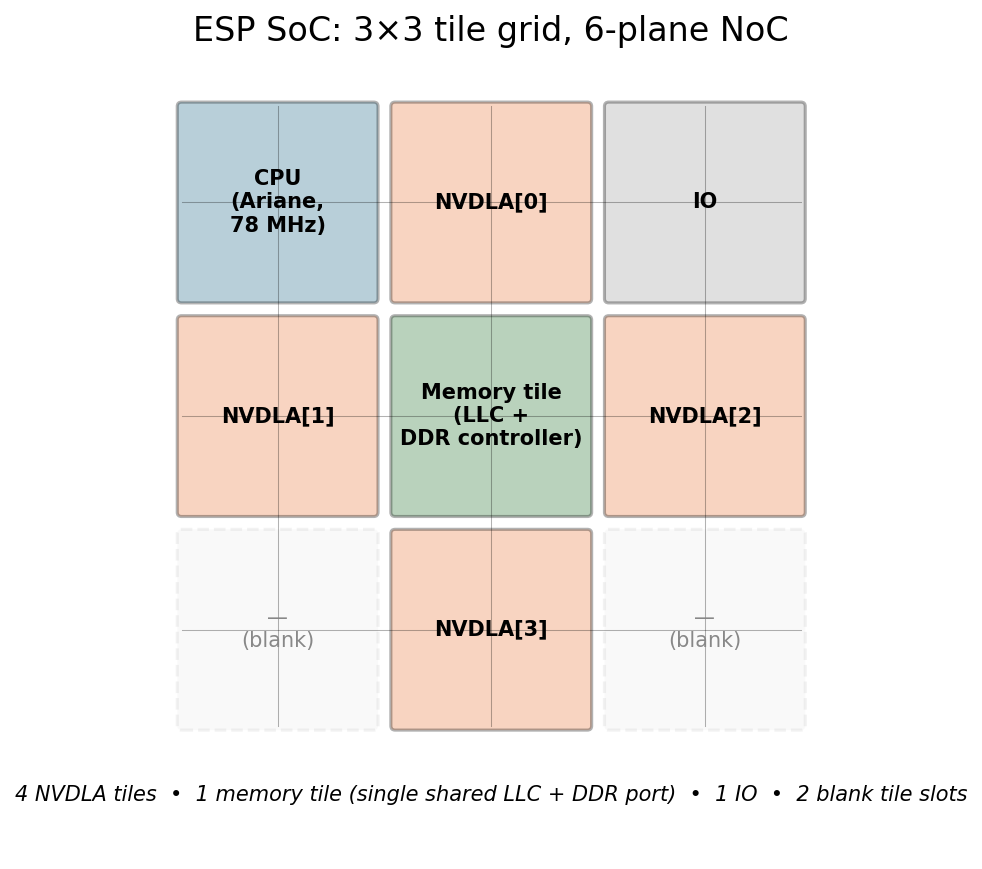
\includegraphics[width=0.95\columnwidth]{figs/architecture.png}
\caption{ESP SoC tile layout. Four NVDLA tiles share a single memory
tile containing the LLC and the DDR controller. All tiles share the
78~MHz base clock.}
\label{fig:arch}
\end{figure}

\subsection{Target Network: ResNet-18}
We chose ResNet-18 as the target. The network contains 18 weighted
layers organized into a stem convolution, four residual stages
(layer1--layer4), each containing two BasicBlocks (Figure
\ref{fig:resnet18}), and a fully-connected head. After deduplicating
shape-equivalent layers, ResNet-18 has \textbf{11 distinct conv
shapes} spanning the full range from input-heavy
(\texttt{conv1}: $7\times7$, 3 input channels, 64 output channels,
$224\times224$ spatial) to weight-heavy
(\texttt{layer4\_3x3}: $3\times3$, 512$\to$512 channels, $7\times 7$
spatial). The model is INT8-friendly, well-studied, and small enough
to validate exhaustively on FPGA.

\begin{figure}[t]
\centering
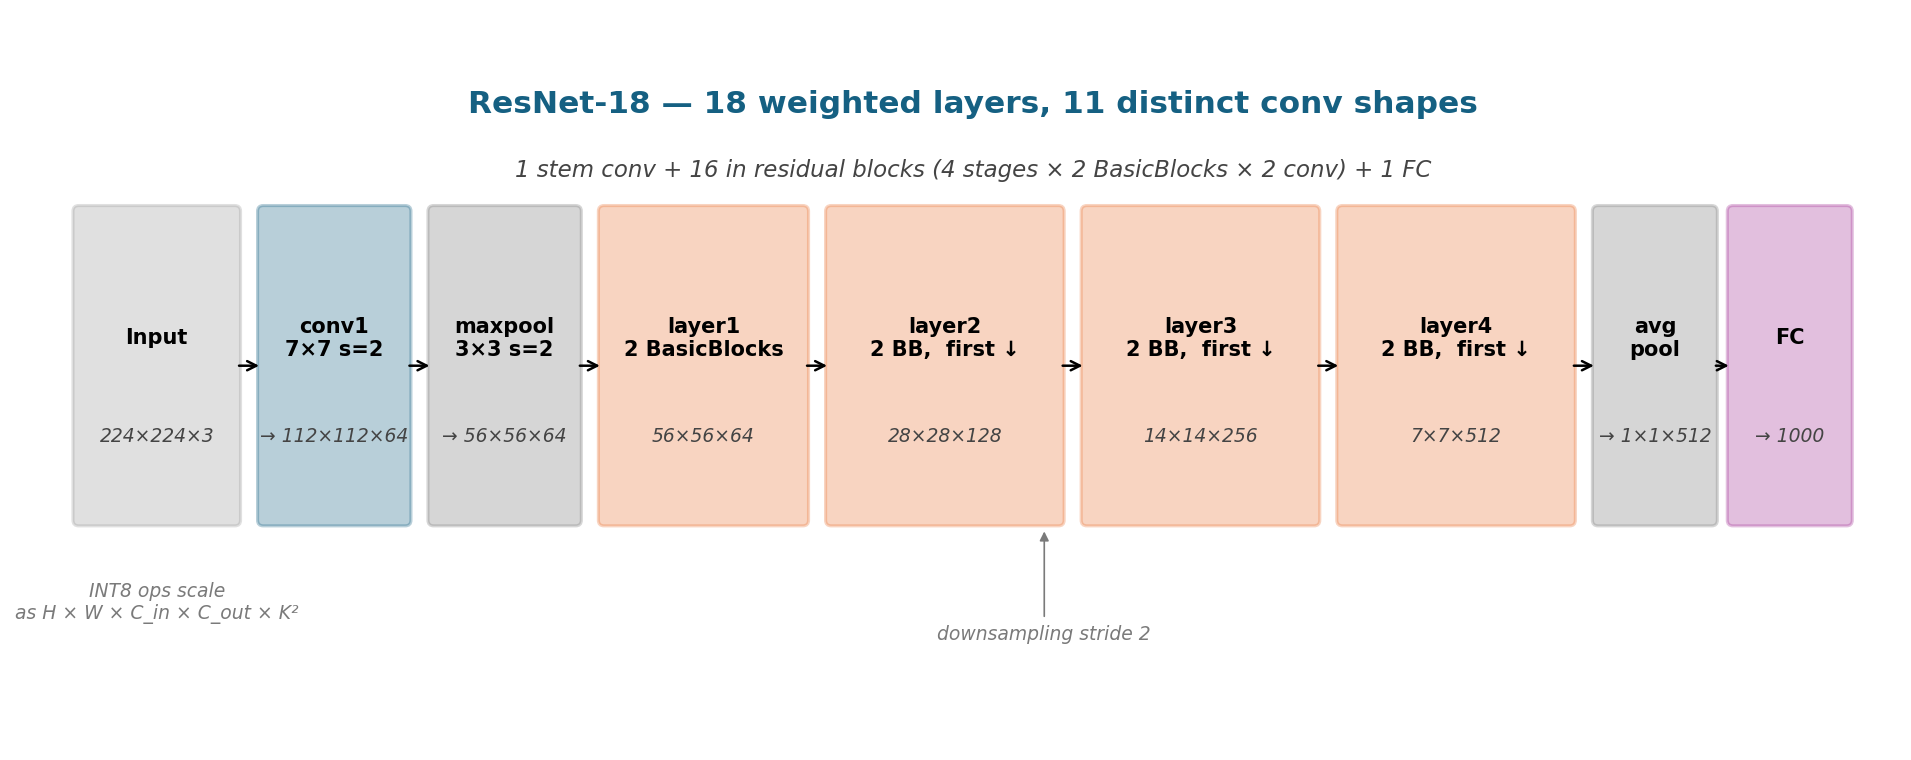
\includegraphics[width=\columnwidth]{figs/resnet18_arch.png}
\caption{ResNet-18 architecture. Four residual stages with progressively
smaller spatial dimensions and larger channel counts produce the wide
range of arithmetic intensities that makes per-layer analysis informative.}
\label{fig:resnet18}
\end{figure}

\subsection{Workflow and Instrumentation}
The end-to-end workflow (Figure~\ref{fig:workflow}) takes a Caffe
network description, runs our \texttt{gen\_resnet18.py} generator to
emit a baseline loadable and $N$ output-channel-split loadables for
each distinct conv shape, stages the loadables into the FPGA's
buildroot sysroot, rebuilds the Linux image, and boots on the FPGA.
On-board, we wrap each \texttt{nvdla\_runtime} invocation with a
small C harness, \texttt{monitor\_run.exe}, that snapshots the ESP
hardware-monitor counters \cite{libmonitors} before and after the run
and emits a 23-column CSV per accelerator tile. Captured counters
include accelerator-tile non-idle cycles (\texttt{acc\_tot\_cycles})
and memory-state cycles (\texttt{acc\_mem\_cycles}) measured at the
NVDLA tile clock, off-chip DRAM write-data beat count
(\texttt{ddr\_words}) measured at the memory-tile clock, per-NoC-plane
inject counts, LLC coherence statistics, and memory-tile DMA request
and response counts.

\begin{figure}[t]
\centering
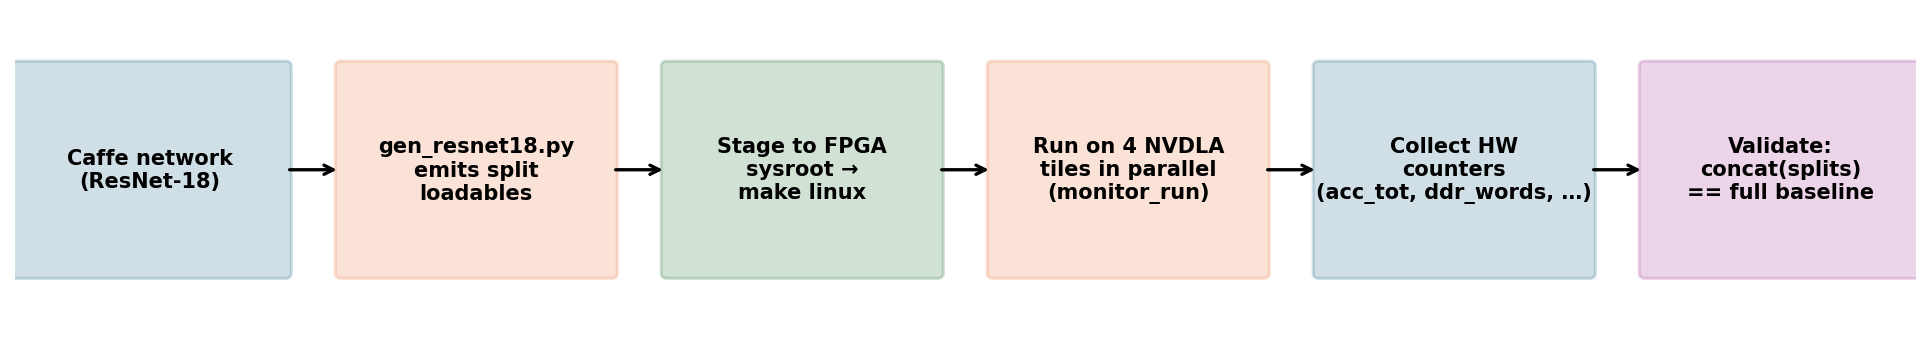
\includegraphics[width=\columnwidth]{figs/workflow.png}
\caption{End-to-end workflow. Compile-time loadable generation,
target-side staging, parallel execution on four NVDLA tiles, and
bit-exact correctness validation.}
\label{fig:workflow}
\end{figure}

All performance numbers reported in this paper come from on-FPGA runs;
none are from simulation.

\subsection{Roofline Sweep}
To diagnose the per-layer performance characteristics, we designed an
auxiliary sweep of 27 isolated single-convolution configurations spanning
arithmetic intensities from 49 to 664 INT8 ops per byte. The
configurations are organized into seven controlled groups (reference,
\texttt{vary\_h}, \texttt{vary\_c}, \texttt{vary\_k}, asymmetric,
output-heavy, weight-heavy). Each group fixes all dimensions except
one, so a trend within a group isolates the effect of varying that
one parameter (spatial size $H$, channel count $C$, kernel size $K$,
or input/output channel asymmetry).


\section{Results}\label{sec:results}

\subsection{Correctness}
For each of the 11 distinct conv shapes in ResNet-18, we ran the
full-layer baseline on one NVDLA tile and the four output-channel-split
loadables in parallel on tiles~0--3, both with the runtime's
\texttt{--rawdump} option enabled, then concatenated the four split
outputs along the channel axis and compared bit-exactly to the
baseline output using \texttt{md5sum}.

\textbf{All 11 layers pass bit-exactly.} The output element counts
match the expected ResNet-18 shapes: 802\,816 values for
\texttt{conv1}, 200\,704 for \texttt{layer1}, 100\,352 for
\texttt{layer2}, 50\,176 for \texttt{layer3}, and 25\,088 for
\texttt{layer4}. We also verified that re-running the same loadable
yields the same \texttt{md5sum}, confirming run-to-run determinism.
Every subsequent timing result operates on known-correct compute.

\subsection{Per-Layer Speedup}
Figure~\ref{fig:headline} compares hardware-cycle costs under
single-tile baseline and 4-way output-channel split. Under 4-way
parallelism, per-tile work runs $3.29\times$ slower for
\texttt{conv1} (22.95~M $\to$ 75.41~M cycles) and $3.20\times$ slower
for \texttt{layer4\_3x3} (9.70~M $\to$ 31.09~M cycles). The
hardware-cycle speedup is approximately $0.30\times$ per tile.
Wall-clock submit time is approximately $4\times$ slower in 4-way
mode for both layers. In every measurement, the FSM-counter ratio
$\textrm{acc\_mem}/\textrm{acc\_tot} \approx 100\%$, with
$\textrm{acc\_tot} - \textrm{acc\_mem} \le 6$ cycles in all cases:
the tile is reported as ``in a memory state'' essentially every cycle.

\begin{figure}[t]
\centering
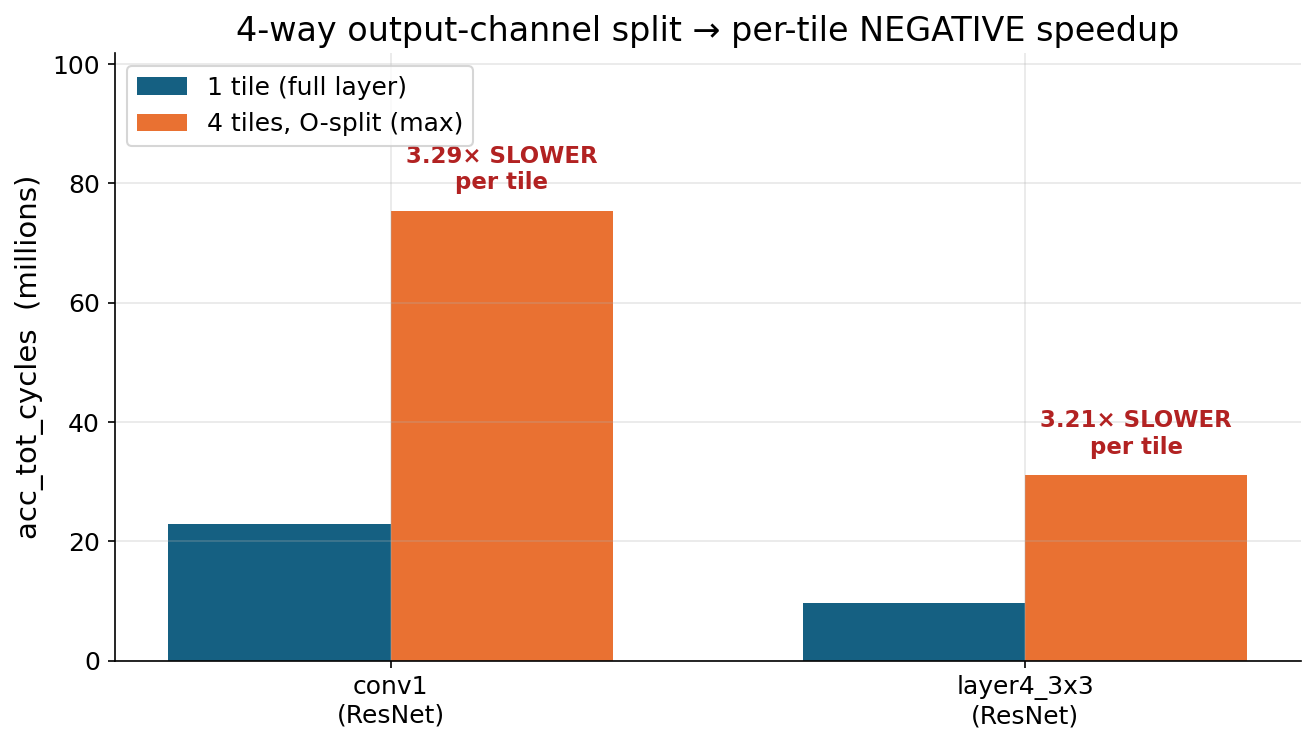
\includegraphics[width=\columnwidth]{figs/headline_slowdown.png}
\caption{4-way output-channel split delivers \emph{negative} per-tile
speedup. Per-tile NVDLA-cycle cost grows by roughly $3.2\times$ in 4-way
mode for both representative layers tested.}
\label{fig:headline}
\end{figure}

\subsection{Roofline Characterization}\label{sec:roofline}
Figure~\ref{fig:roofline} plots achieved compute throughput
($\textrm{ops}/\textrm{NVDLA-cycle}$) versus arithmetic intensity
($\textrm{ops}/\textrm{byte}$) for all 27 single-tile configurations.
Three ceilings are drawn. The horizontal \textbf{compute peak} at
128 ops/cy is set by \texttt{nv\_small\_fpga}'s 64 INT8 MACs and 2 ops
per MAC. The sloped \textbf{NoC bandwidth peak} at $8\,\textrm{B/cy} \times
\textrm{AI}$ is set by the 64-bit-wide DMA NoC plane at the tile
clock~\cite{esp_iccad}. The red dotted \textbf{per-tile achievable}
line at approximately $0.49\,\textrm{B/cy} \times \textrm{AI}$ is a
model of what one NVDLA tile can sustain given the platform's burst
size and outstanding-transaction limits; we derive this ceiling in
Section~\ref{sec:rootcause} and treat the precise slope as an
order-of-magnitude estimate, not a calibrated measurement.

\begin{figure}[t]
\centering
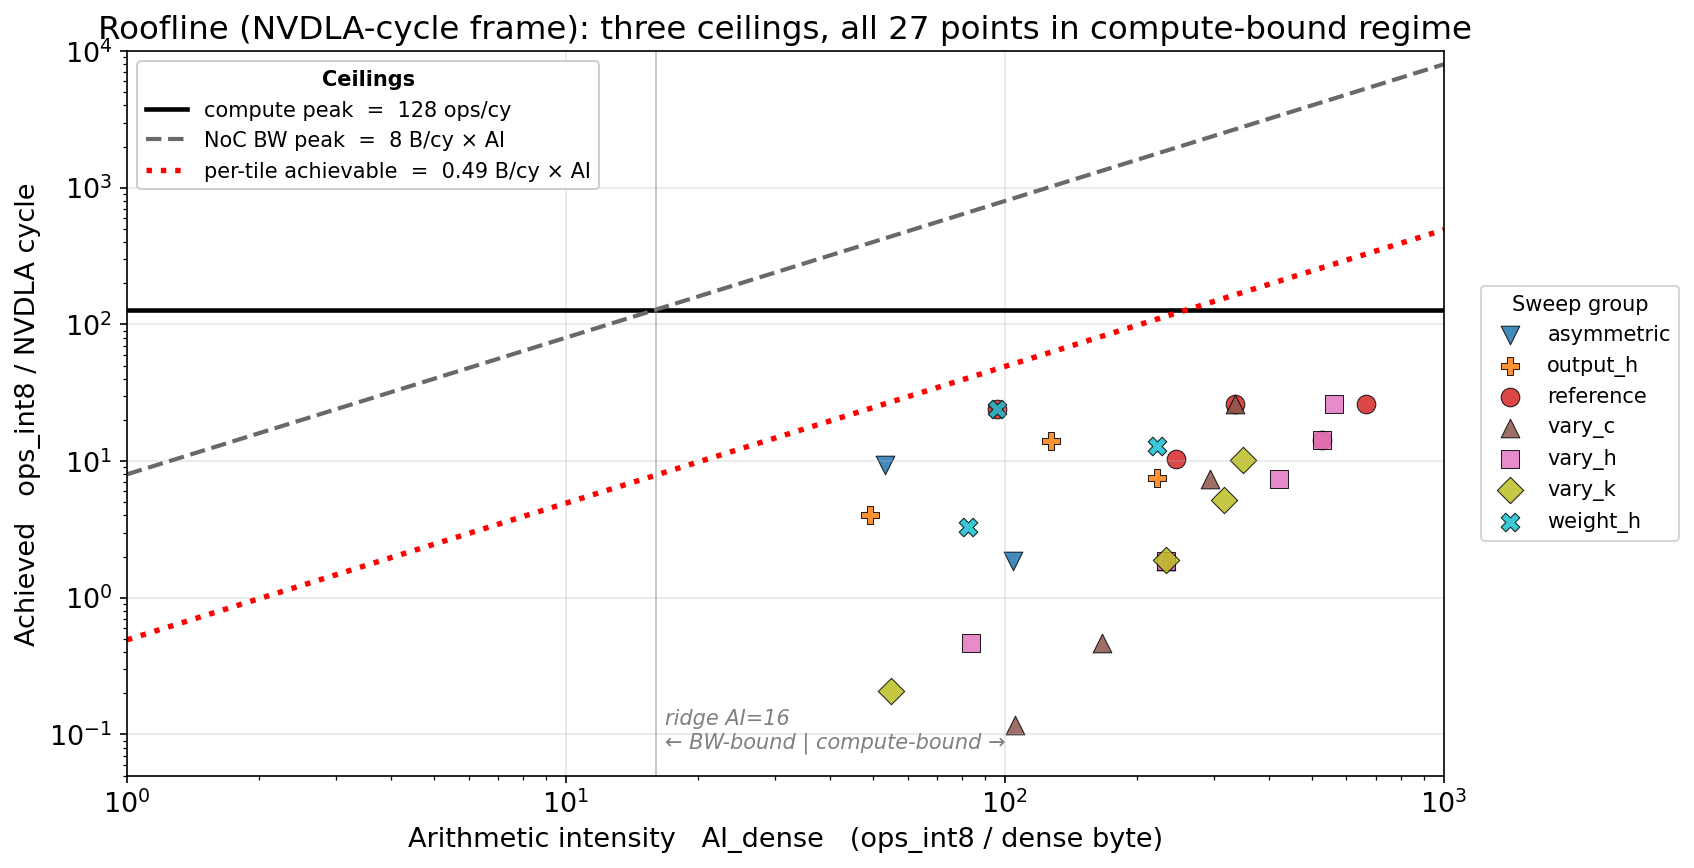
\includegraphics[width=\columnwidth]{figs/roofline_unitclean.png}
\caption{Roofline characterization across 27 single-conv configurations.
All workloads have $\textrm{AI} > 16$ (the ridge point), so classical
roofline analysis predicts they should be compute-bound. They are not:
the best achieved throughput is 26.3 ops/cy, only 20.6\% of compute
peak. Points cluster well below all three ceilings, with most workloads
sitting in the latency-stalled regime characterized by the per-tile
achievable line.}
\label{fig:roofline}
\end{figure}

Every workload has arithmetic intensity well above the
$\textrm{AI}=16$ ridge where the NoC BW ceiling crosses compute peak.
Classical roofline analysis therefore predicts every workload should
be compute-bound. They are not: the best single-tile workload achieves
only 26.3 ops/cycle, $20.6\%$ of compute peak. The cluster of points
sits between the NoC BW ceiling and the per-tile achievable line. The
data is fundamentally inconsistent with a bandwidth-saturated
interpretation: the NoC has slack and DRAM has slack, yet performance
is far from compute peak.

\subsection{Direct Evidence for Latency Bounding}\label{sec:varyh}
Figure~\ref{fig:varyh} isolates the spatial dimension $H$ while
holding $C_{in}=C_{out}=64$, $K=3$, and $\textrm{stride}=1$ fixed.
Both effective DRAM throughput
($\textrm{ddr\_words}\cdot 8/\textrm{acc\_tot}$) and achieved
$\textrm{ops}/\textrm{cycle}$ grow monotonically with $H$, by roughly
$6\times$ as $H$ grows $16\times$. The mechanism is straightforward:
larger spatial outputs produce longer sequential bursts that the
DMA engine can pipeline, amortizing per-request round-trip latency
over more useful bytes. This is the canonical signature of a
latency-bound rather than bandwidth-bound system.

\begin{figure}[t]
\centering
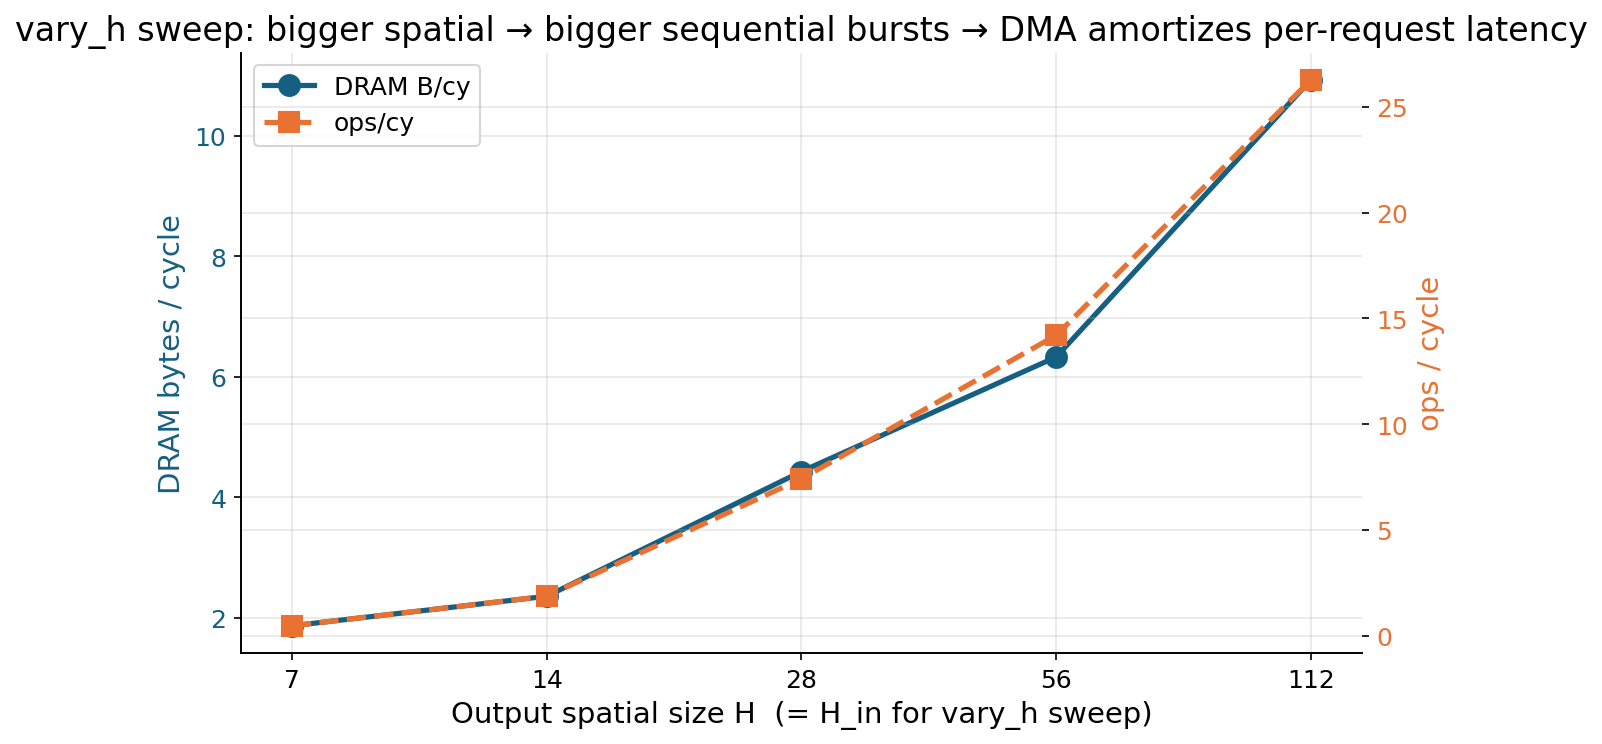
\includegraphics[width=\columnwidth]{figs/vary_h_trend.png}
\caption{\texttt{vary\_h} sweep with all other parameters fixed.
Effective throughput grows monotonically with output spatial size,
consistent with latency amortization across larger sequential bursts.}
\label{fig:varyh}
\end{figure}

\subsection{Multi-Tile Contention}
To distinguish the 4-way slowdown of output-channel split from any
generic property of running four tiles in parallel, we ran four
\emph{independent} (non-cooperative) copies of the same loadable on
tiles 0--3 simultaneously and compared per-tile timing against the
single-tile baseline. We selected three workloads representing
different single-tile regimes
(Figure~\ref{fig:contention}). The result is striking: all three
workloads exhibit the same $3.5\textrm{--}3.9\times$ per-tile
slowdown, irrespective of whether they were write-pipelined or
read-latency-stalled in single-tile mode. Aggregate SoC DRAM-write
throughput in 4-tile mode is only $1.04\textrm{--}1.14\times$ that
of single-tile mode, far short of the ideal $4\times$ scaling.

\begin{figure}[t]
\centering
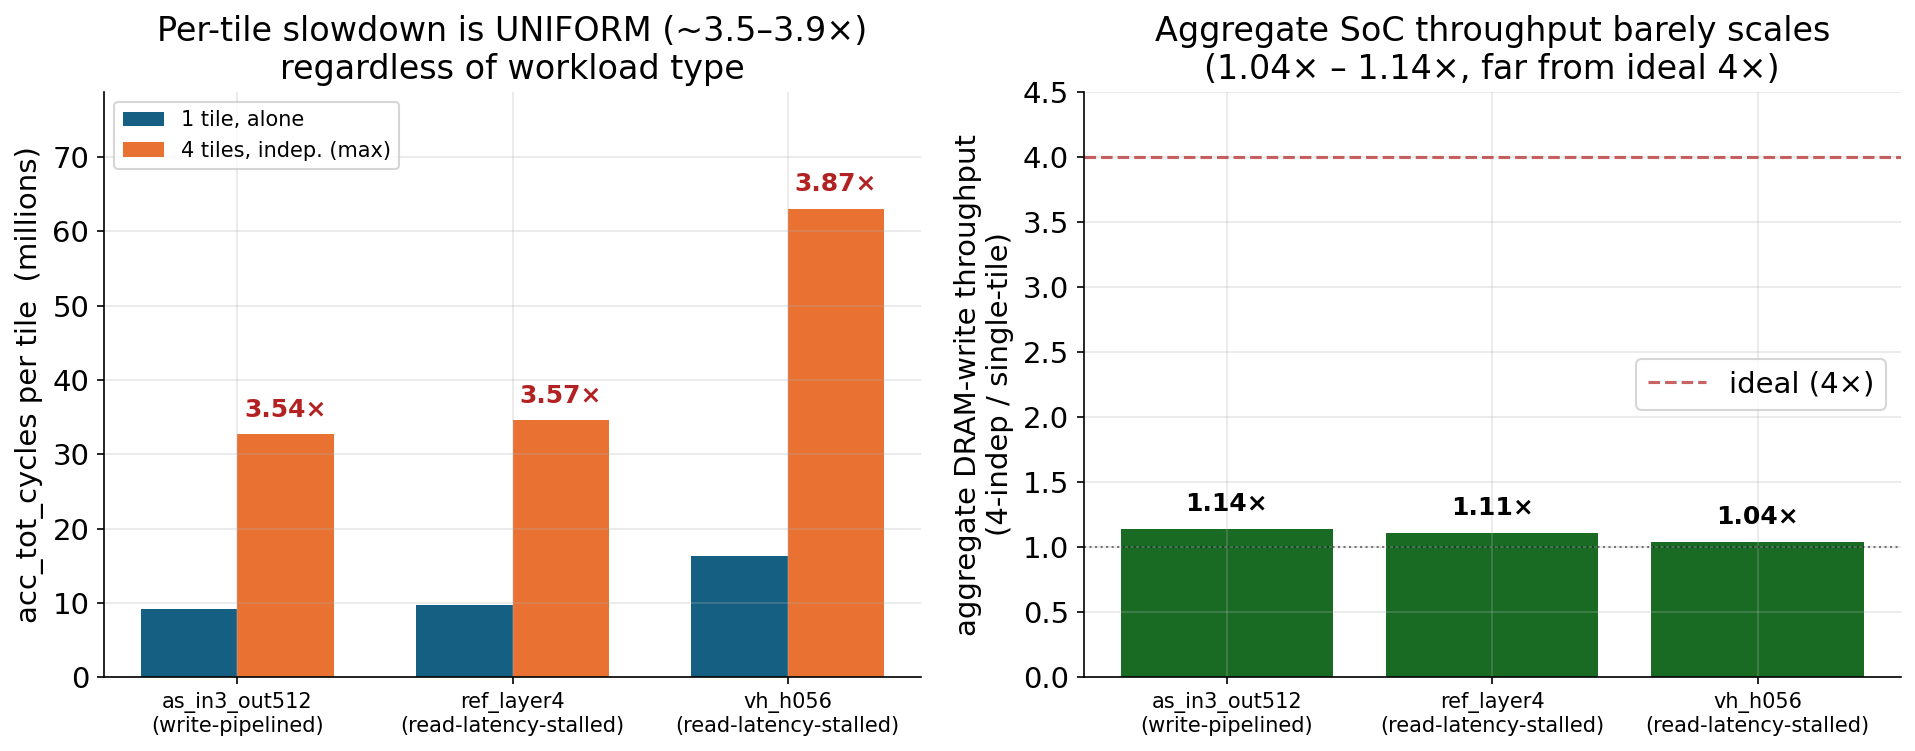
\includegraphics[width=\columnwidth]{figs/contention.png}
\caption{Multi-tile contention experiment: four independent copies of
the same loadable on four tiles. Per-tile slowdown is uniform at
$3.5\textrm{--}3.9\times$ regardless of workload type. Aggregate
SoC throughput barely scales above single-tile baseline.}
\label{fig:contention}
\end{figure}

The implication is important: the 4-way slowdown observed for
output-channel split is not a property of that partitioning strategy.
It is a property of running four tiles in parallel against a shared
memory subsystem.


\section{Root-Cause Analysis}\label{sec:rootcause}

The combination of single-tile results in
Section~\ref{sec:roofline}--\ref{sec:varyh} and the contention
experiment together point at a single mechanism with two cooperating
parts.

\subsection{Burst-Size Mismatch}
The ESP NoC DMA plane is 64 bits wide and the
\texttt{axislv2noc} bridge encodes AXI burst length in a 9-bit field
(AXI \texttt{awlen}+1), supporting up to 256-beat bursts, i.e.\ a
maximum payload of 2048 B per AXI transaction~\cite{esp_iccad}.
NVDLA's \texttt{nv\_small\_fpga} configuration, however, issues
4-beat $\times$ 8-byte bursts, i.e.\ \textbf{32 B per AXI
transaction} (Figure~\ref{fig:burst}). The maximum burst length in
the upstream NVDLA spec is 1 or 4 beats only; widening this
requires either a different NVDLA configuration with a wider data
path (\texttt{nv\_medium\_512} at 64 B, \texttt{nv\_large} at 128
B) or RTL changes to NVDLA itself. The result is a $\sim 64\times$
efficiency loss on per-transaction overhead at the NoC, and---more
importantly---a $\sim 64\times$ multiplier on the number of
transactions required to move a given amount of data.

\begin{figure}[t]
\centering
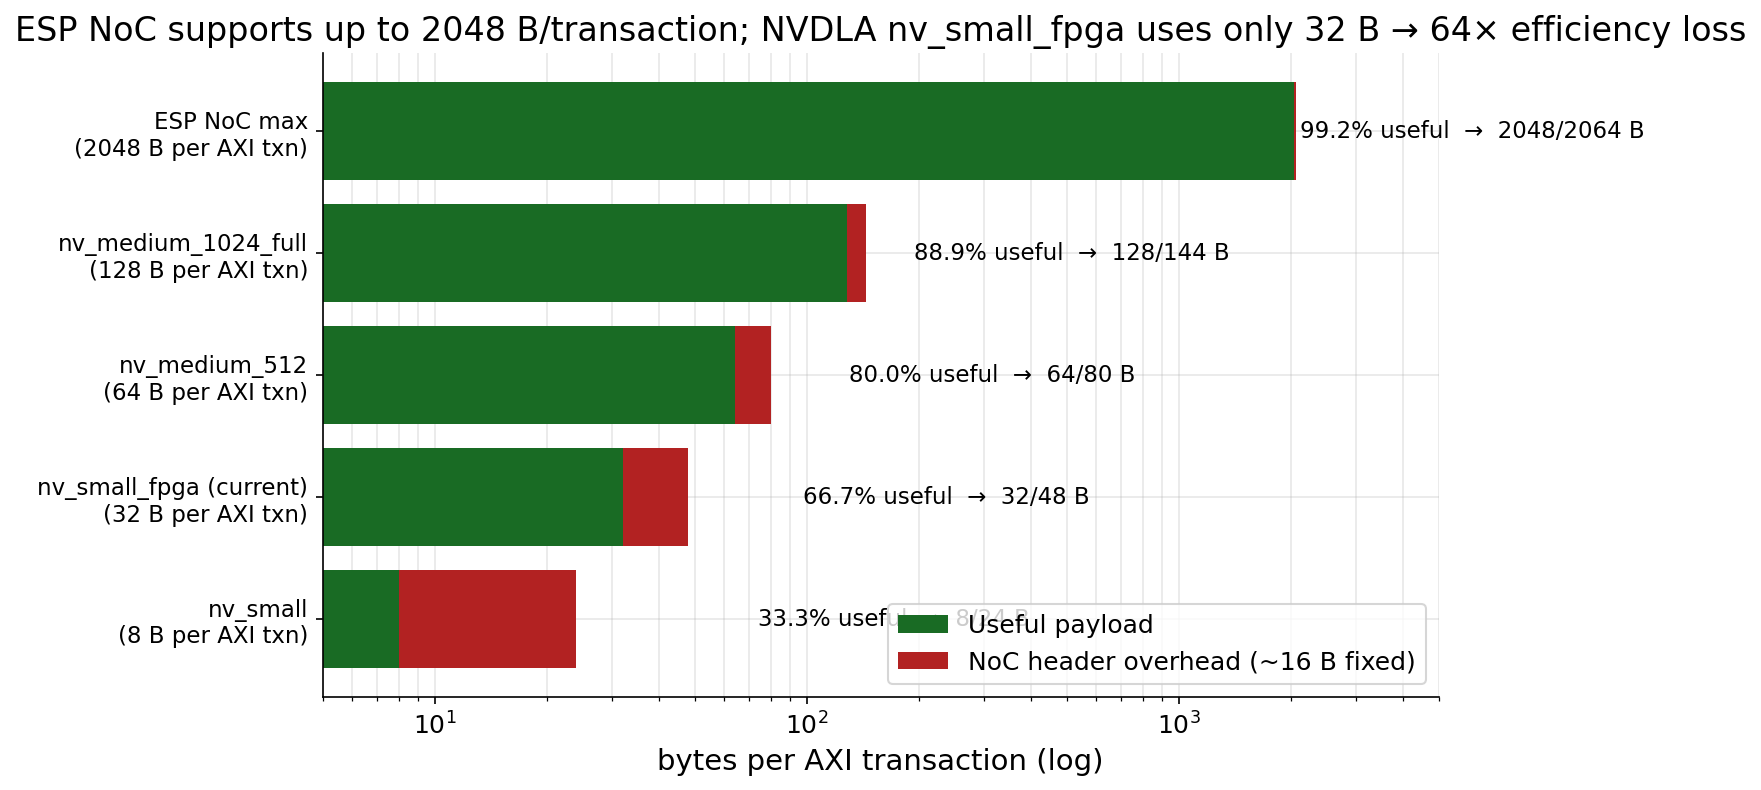
\includegraphics[width=\columnwidth]{figs/burst_mismatch.png}
\caption{Payload per AXI transaction across NVDLA configurations and
the ESP NoC maximum. Our \texttt{nv\_small\_fpga} build uses
4-beat $\times$ 8-byte = 32 B bursts, $64\times$ smaller than the
NoC's 2048-byte capacity.}
\label{fig:burst}
\end{figure}

\subsection{Outstanding-Transaction Serialization}
ESP's accelerator-to-NoC bridge permits only a single outstanding
AXI transaction per master at a time. NVDLA can in principle issue
multiple memory requests concurrently from its CDMA, CACC, and SDP
units, but the ESP integration layer serializes them at the NoC
boundary. Round-trips are not pipelined; the next request can only
fire after the previous response has returned.

\subsection{Combined Effect}
The combination of small bursts and single-outstanding-transaction
serialization sets the per-tile achievable bandwidth ceiling:
\[
B_{\textrm{per-tile}} \approx \frac{\textrm{payload per AXI txn}}
{\textrm{cycles per AXI txn round-trip}}.
\]
For a working-bench estimate we used a round-trip of 65 cycles,
giving $32\,\textrm{B}/65\,\textrm{cy} \approx 0.49$ B/NVDLA-cycle
$\approx 38$ MB/s/tile, which is the slope of the red dotted line
on the roofline plot. \textbf{However, this number is a coarse
estimate that we did not directly measure on our bitstream.}
Section~\ref{sec:limits} discusses this in detail.

Under multi-tile parallelism, each tile's round-trip is further
elongated because the four tiles share a single memory tile and
its single LLC/DRAM port. With four tiles each carrying one
outstanding transaction, requests serialize at the memory-tile
arbiter; each tile's effective round-trip grows by roughly
$N\times$. This explains the observed
$3.5\textrm{--}3.9\times$ per-tile slowdown
uniformly across workload types: the binding constraint is the
shared serialization slot, not any property of the partitioning
strategy or any layer-specific arithmetic profile.


\section{Limitations}\label{sec:limits}

Every result in this paper is from on-FPGA measurements, not
simulation. However, the FPGA was shared with other students under
a scheduling system that did not always align with our experimental
plans, and several sessions ended early because the JTAG link became
unstable or the board could not be re-programmed on time. We are
therefore explicit about what our measurements can and cannot support.

\subsection{The 65-Cycle Round-Trip Estimate}\label{sec:65cy}
The most quantitative limitation concerns the per-AXI-transaction
round-trip in Section~\ref{sec:rootcause}. \textbf{The value 65
cycles is not an empirical measurement on our SoC}---it is the
midpoint of a 50--70 cycle reference range cited by our TAs during
a meeting on May~6, taken from a separate dummy-accelerator
characterization they had performed on a similar ESP SoC. During
the final-presentation Q\&A the instructor suggested that 20--30
cycles would be more reasonable for this platform, although he was
not certain. Either estimate is consistent with our measurements;
a direct on-bitstream characterization would be required to settle
the exact value.

Two observations bound the uncertainty. First, the qualitative
story is invariant under any plausible round-trip value. Whether
the true number is 25, 50, or 70 cycles, the per-tile achievable
ceiling lies far below both the NoC bandwidth ceiling and the
compute peak; the cluster of 27 points in Figure~\ref{fig:roofline}
sits well below all three ceilings; and the $3.5\textrm{--}3.9\times$
uniform multi-tile slowdown is unchanged. The root-cause attribution
to small bursts $+$ outstanding-transaction serialization is
robust. Second, our measured throughput numbers actually fall
\emph{below} the line predicted by the 65-cycle model, not at or
above it---which suggests that additional per-invocation overhead
inside NVDLA's pipeline (descriptor processing, CBUF fill,
completion accounting) compounds the round-trip cost rather than
shortens it. A 20--30 cycle round-trip alone would predict even
higher achievable throughput than we observed, so the discrepancy
points to further structural overhead beyond the round-trip
itself. Resolving the exact decomposition is item~R1 in
Section~\ref{sec:future}.

\subsection{Counters That Did Not Fire or Were Not Read}
Three measurement gaps affect what we can definitively claim.
First, the \texttt{ddr\_words} hardware counter fires only on the
AXI W-channel handshake at the memory tile, so it counts only
\emph{writes}; NVDLA's weight reads, input reads, and intermediate
activation reads are invisible to it. Second, the
per-NVDLA-tile NoC inject counters did not fire for bulk-data
traffic in our bitstream: the monitored signal is on the tile's
local NoC router port, and NVDLA's DMA-to-NoC bridge in the
third-party tile wrapper appears to take a path that does not
assert that signal---NVDLA tiles register only $\sim 50\textrm{--}200$
packets per run on plane~5 (likely register MMIO), while the CPU
tile records hundreds of thousands of plane-1 packets in the same
window. Third, NVDLA's own internal performance registers
(the \texttt{CDMA\_PERF\_*} and \texttt{CACC\_PERF\_*} stall
counters) were not read; this would have required a small
\texttt{/dev/mem} mmap helper into the NVDLA register window
that we did not complete before FPGA access was lost.

\subsection{Measurements Not Performed}
We did not run end-to-end ResNet-18 inference with chained
split-layer execution. Per-layer correctness is verified for all
11 layers; per-tile timing data is collected for two layers
(\texttt{conv1} and \texttt{layer4\_3x3}). End-to-end inference
would require automatic activation reconstruction at every
split$\to$merge boundary---engineering automation rather than new
methodology. We did not run alternative split strategies
(input-channel, batch, input-spatial); output-channel was the
diagnostic-priority target. We did not collect 2-tile or 3-tile
contention data; only $N=1$ and $N=4$ points were captured.

Despite these gaps, the data is internally consistent and supports
the conclusions we draw. Per-layer correctness is verified
exhaustively; multi-tile slowdown is confirmed across both
output-channel-split and independent-copy workloads; the roofline
cluster is consistent with a latency-bound regime; and the
structural causes (32-byte bursts, single outstanding transaction)
are directly readable from the RTL and the NVDLA configuration
files.


\section{Future Work}\label{sec:future}

We outline three concrete experiments, in increasing order of cost,
that would tighten or extend the present result.

\noindent\textbf{R1: 2-tile and 3-tile contention sweep, plus NVDLA
internal CDMA stall counters.} No re-synthesis is needed. With
roughly one hour of FPGA time and a small
\texttt{/dev/mem} helper, this would:
\textbf{(a)} discriminate gradual NoC contention from single-point
serialization by measuring per-tile \texttt{acc\_tot} at $N=2,3,4$;
\textbf{(b)} give a direct measurement of read-side and weight-side
stall cycles inside NVDLA, which would pin down the actual
round-trip time on our bitstream and resolve the 65~cycle vs.
20--30 cycle uncertainty discussed in Section~\ref{sec:65cy}.

\noindent\textbf{R2: Re-synthesize with \texttt{nv\_small\_256\_full}.}
This NVDLA configuration retains the 32~B burst size but adds a
second NVDLA memory port (\texttt{SECONDARY\_MEMIF\_ENABLE}). The
test isolates whether NVDLA's per-tile AXI port is the binder; if
so, doubling the per-tile port count should approximately halve
the per-tile time.

\noindent\textbf{R3: Re-synthesize with \texttt{nv\_medium\_512} or
\texttt{nv\_large}.} These configurations widen the AXI data path
to 128 or 256 bits, raising per-AXI-transaction payload to 64 or
128 B respectively. The test directly addresses the burst-size
half of the root cause. We expect that doubling the per-transaction
payload should approximately double the per-tile achievable
bandwidth, modulo unchanged per-transaction round-trip latency.

Other follow-on directions include increasing \texttt{SOC\_NMEM}
beyond 1 (more memory tiles to relieve LLC-port serialization),
implementing input-channel split with partial-sum reduction over the
NoC, and developing the automatic chained-inference runtime
required for end-to-end ResNet-18 execution.


\section{Conclusions}\label{sec:concl}

We have built, verified, and characterized a working
compile-time output-channel-splitting workflow for ResNet-18 on
the ESP-NVDLA platform. The implementation is correct: all 11
distinct conv shapes pass bit-exact validation across baseline
and 4-way splits. The performance characterization yields a
negative but informative result: 4-way splits deliver an inverse
speedup of approximately $0.30\times$ per tile, uniformly across
layer types and across non-cooperative tile usage.

The root cause is a combination of two structural properties of
the platform---NVDLA's 32~B AXI bursts and ESP's
single-outstanding-transaction serialization---compounded by a
single shared memory tile. These mechanisms together produce a
latency-stalled regime in which DRAM bandwidth has substantial
slack but per-tile throughput is bounded by per-AXI-transaction
round-trip cost. Under multi-tile parallelism, the shared
memory-side serialization slot makes per-tile time grow linearly
with tile count, so the partitioning strategy cannot deliver
parallel speedup regardless of how cleanly the work is split.

The negative speedup is a property of the platform
\emph{configuration}, not of the partitioning algorithm. The
specific architectural knobs that would unlock parallel speedup
---wider NVDLA AXI bursts, deeper outstanding-transaction queues,
multiple memory tiles---are identifiable and quantifiable from
the present data. The follow-on experiments outlined in
Section~\ref{sec:future} would either confirm these targets or
identify any remaining structural limits.


\begin{thebibliography}{1}

\bibitem{simba}
Y. S. Shao, J. Clemons, R. Venkatesan, B. Zimmer, M. Fojtik, N. Jiang,
B. Keller, A. Klinefelter, N. Pinckney, P. Raina, S. G. Tell, Y.
Zhang, W. J. Dally, J. Emer, C. T. Gray, B. Khailany, and S. W.
Keckler, ``Simba: Scaling Deep-Learning Inference with Multi-Chip-
Module-Based Architecture,'' in \emph{Proceedings of the 52nd
Annual IEEE/ACM International Symposium on Microarchitecture
(MICRO)}, 2019.

\bibitem{nvdla_web}
NVIDIA Corporation, ``NVDLA Open Source Project,''
\url{http://nvdla.org/}, Accessed: 2026.

\bibitem{esp_iccad}
P. Mantovani, D. Giri, G. Di Guglielmo, L. Piccolboni, J. Zuckerman,
E. G. Cota, M. Petracca, C. Pilato, and L. P. Carloni, ``Agile SoC
Development with Open ESP,'' in \emph{IEEE/ACM International
Conference on Computer Aided Design (ICCAD)}, 2020.

\bibitem{esp_vlsid}
L. P. Carloni, ``ESP: The Open-Source SoC Platform,'' in
\emph{International Conference on VLSI Design and International
Conference on Embedded Systems (VLSID)}, 2020.

\bibitem{survey_accel}
A. Reuther, P. Michaleas, M. Jones, V. Gadepally, S. Samsi, and J.
Kepner, ``Survey of Machine Learning Accelerators,'' in \emph{IEEE
High Performance Extreme Computing Conference (HPEC)}, 2020.

\bibitem{libmonitors}
System-Level Design Group at Columbia University, ``Monitors API
Guide,'' \emph{ESP Documentation}, 2026. [Online]. Available:
\url{https://www.esp.cs.columbia.edu/docs/monitors_api/monitors_api-guide/}

\bibitem{esp_nvdla_guide}
System-Level Design Group at Columbia University, ``Guide -- How
to: integrate a third-party accelerator (e.g. NVDLA),''
\emph{ESP Documentation}, Aug. 2021. [Online]. Available:
\url{https://www.esp.cs.columbia.edu/docs/thirdparty_acc/thirdparty_acc-guide/}

\end{thebibliography}

\end{document}
